\documentclass{beamer}

\usepackage[utf8]{inputenc}
\usepackage{default}
\usepackage{graphicx}
\usepackage{bbding}


% TODO Learn what this does
% source
% http://tex.stackexchange.com/questions/15952/layout-of-multiple-lines-footnotes
% this is a way to adjust foot note so it can be cutted into multiple lines
\makeatletter
\renewcommand\@makefntext[1]{\tiny\rightskip=25em\hskip0em\@makefnmark#1}
\makeatother

\makeatletter
\newcommand*{\rom}[1]{\expandafter\@slowromancap\romannumeral #1@}
\makeatother


% shows how to change default (blue) colours in the default beamer theme
% found here: http://joerglenhard.wordpress.com/tag/latex/
\definecolor{WaterlooRed}{RGB}{145,11,46}
\setbeamercolor{title}{fg=WaterlooRed}
\setbeamercolor{frametitle}{fg=WaterlooRed}
\setbeamercolor{structure}{fg=WaterlooRed}

% adds logo in the footer
\logo{
\includegraphics[scale=.25]{img/csuow}}

\title[]{MicroFuge: A Middleware Approach to Providing Performance Isolation in Cloud Storage Systems}
\author[Akshay Singh, Xu Cui, Benjamin Cassell, Bernard Wong and Khuzaima Daudjee]{Akshay Singh, \textbf{Xu Cui}, Benjamin Cassell, Bernard Wong and Khuzaima Daudjee}
\institute{
\includegraphics[scale=0.25]{img/UniversityOfWaterloo_logo_vert_rgb.png}}
\date{{\tiny\today}}


% my macros
\newcommand{\myv}{\vspace{3 mm}}


\begin{document}

\begin{frame}
  \titlepage
\end{frame}


%% \begin{frame}
  %% \frametitle{Cloud Computing}

  %% Cloud computing allows us to share resources effectively at virtualized
  %% level, but at the same time we are sharing the physical resources and
  %% this comes at the cost of reduced isolation between tenants.


  %% \centering
  %% 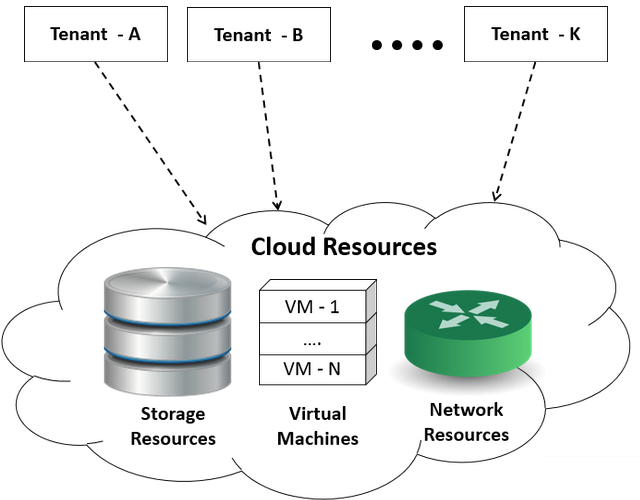
\includegraphics[scale=0.26]{img/icdcs1.png}

%% \end{frame}


\begin{frame}
  \frametitle{Storage Resources in Cloud Datacenters}
\vspace{-5 mm}
    \begin{itemize}
    \item Cloud computing allows sharing of resource at the cost of reduced isolation.
      \newline
    \item Unlike memory, storage system is more affected by performance interference.
      \newline
      \begin{itemize}
      \item Different access patterns by different clients.
        \newline
      \item Various kinds of workloads.
      \end{itemize}
    \end{itemize}
\end{frame}

\begin{frame}
  \frametitle{A Typical Cloud Scenario}
  %% \vspace{5 mm}
  \begin{itemize}

  \item A HTTP request may require 35 database lookups.
    \begin{itemize}
      \myv
    \item Source: Nathan Farrington and Alexey Andreyev, Facebook’s Data Center Network Architecture.
      \myv
    \item Response time can add up quickly.
    \end{itemize}
    \myv
  \item Latency matters.
    \myv
  \item Predictable performance is desired.
    %% \centering
  \end{itemize}

\end{frame}

\begin{frame}
  \frametitle{Implications of Performance Isolation}
  \begin{itemize}
  \item Disk sharing can be troublesome for performance.
    \myv
  \item Clients want to have the performance as if there is no sharing.
    \vspace{-2.5 mm}
  \item Dedicated disks.
    \myv
  \item Meet clients' response time requirements.
    \begin{itemize}
      \myv
      \item Request deadlines.
        \myv
      \item \(\text{Meeting deadlines} \rightarrow \text{Provides Performance Isolation.}\)
    \end{itemize}
  \end{itemize}
\end{frame}


\begin{frame}
  \frametitle{From a Customer's Point of View}
\myv
%% \vspace{10 mm}
  \begin{itemize}
  \item Requests may have stringent response time requirements.
    \myv
  \item Other requests may be able to tolerate high latencies.
    \begin{itemize}
    \item e.g. recommendation system.
    \end{itemize}
    \myv
  \item Need to capture desired response time of requests.
    \myv
  \item A comprehensible metric
    \begin{itemize}
    \item Request deadlines.
    \end{itemize}
  \end{itemize}
\vspace{-5 mm}
  \begin{figure}
    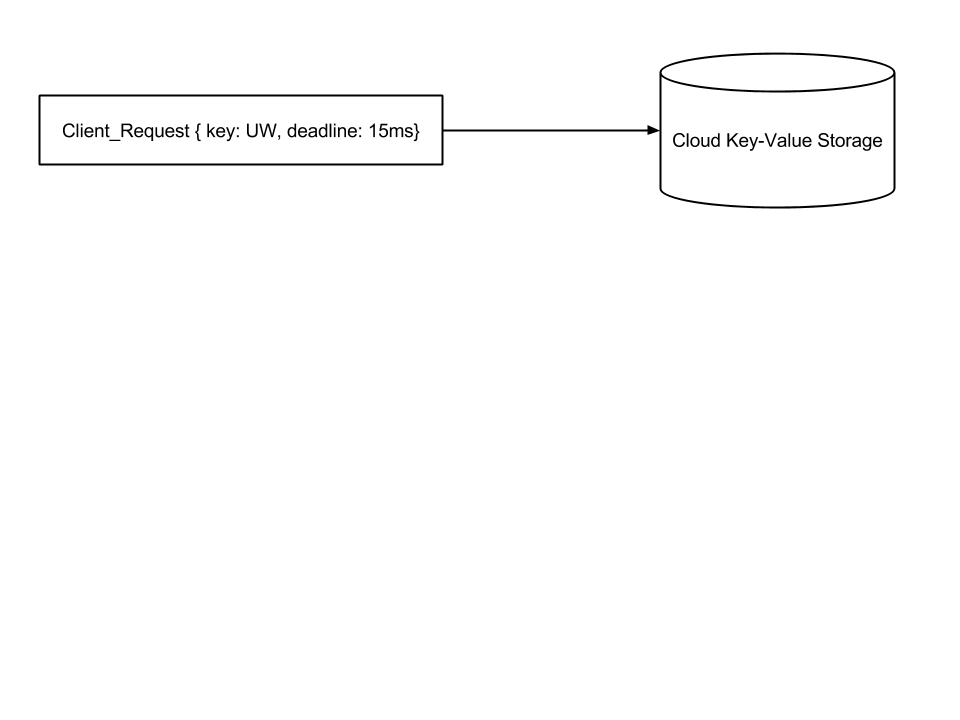
\includegraphics[scale=0.35]{img/Request_Deadline_Example.png}
  \end{figure}
\end{frame}

\begin{frame}
  \frametitle{Middleware Approach}
  \begin{itemize}
    \item Many cloud storage systems - hard to modify.
      \myv
    \item Memcached - A popular middleware.
      \begin{itemize}
      \item Reduces response times.
      \item Deadline oblivious - can't distinguish different response time
        requirements.
      \end{itemize}
      \myv
    \item Similar approach to Memcached, use deadline-aware middleware to
      improve performance isolation.
  \end{itemize}

\end{frame}


%% \begin{frame}
  %% \frametitle{Agenda}
  %% \begin{itemize}
  %% \item[\Checkmark] Background and Motivation
  %% \item MicroFuge
    %% \begin{itemize}
    %% \item Deadline Cache
    %% \item Deadline Scheduler
    %% \end{itemize}
  %% \item Evaluation
  %% \item Conclusion
  %% \end{itemize}
%% \end{frame}


\begin{frame}
  \frametitle{Design Goals of MicroFuge}
  \vspace{-5 mm}
    \begin{itemize}
    \item Meet client requirements despite of performance interference.
      \begin{itemize}
        \myv
      \item Capture response time requirements with request deadlines.
        \myv
      \item Meet request deadlines.
        \myv
      \item Self-adapts to the performance of the underlying storage
        system.
      \end{itemize}
    \myv
    \item Easy adoption - middleware approach.
      \myv
    \item Follow the client-driven, decentralized design.
    \end{itemize}
\end {frame}


%% xcuiTODO: make picture better
\begin{frame}
  \frametitle{MicroFuge Overview (1)}
  %% \begin{itemize}
  %% \item A distributed caching and scheduling middleware that provides
    %% performance isolation.
  \begin{center}
  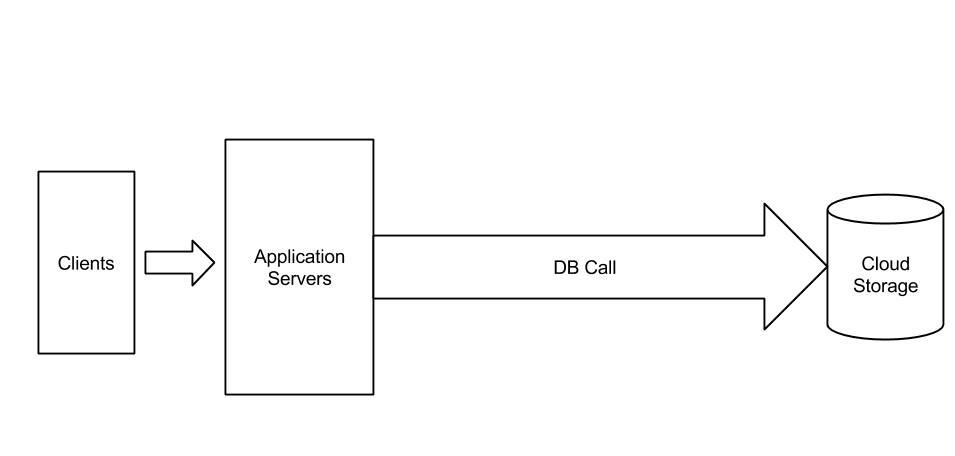
\includegraphics[scale=0.32]{img/MF_FULL_NEW_1.png}
  \end{center}
  %% \end{itemize}
\end{frame}

\begin{frame}
  \frametitle{MicroFuge Overview (2)}
  %% \begin{itemize}
  %% \item A distributed caching and scheduling middleware that provides
    %% performance isolation.
  \begin{center}
  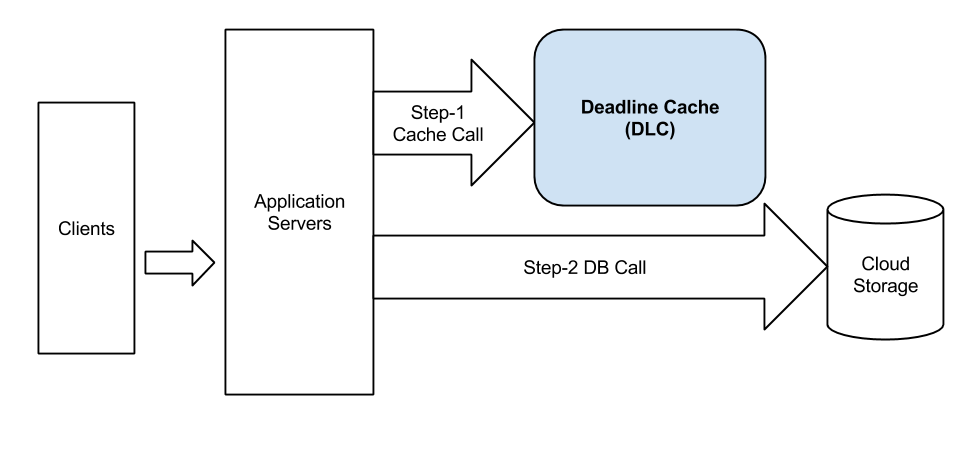
\includegraphics[scale=0.32]{img/MF_FULL_NEW_2.png}
  \end{center}
  %% \end{itemize}
\end{frame}

\begin{frame}
  \frametitle{MicroFuge Overview (3)}
  %% \begin{itemize}
  %% \item A distributed caching and scheduling middleware that provides
    %% performance isolation.
  \begin{center}
  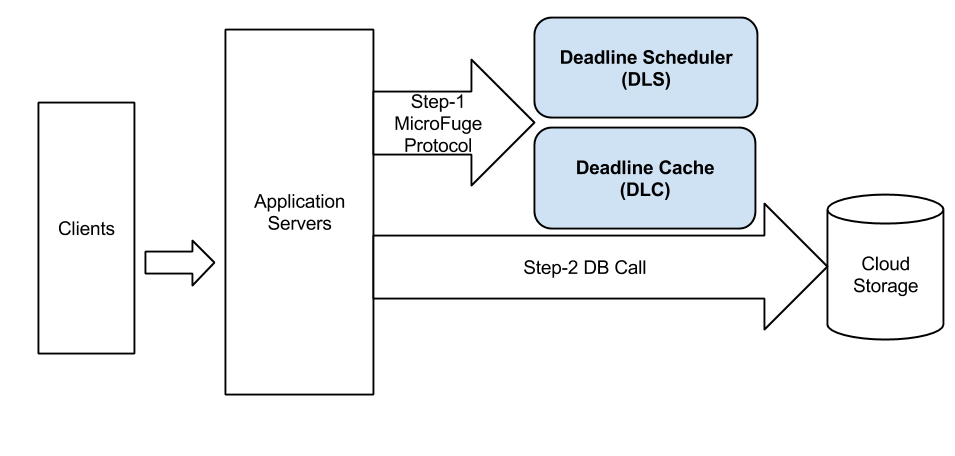
\includegraphics[scale=0.32]{img/MF_FULL_NEW_3.png}
  \end{center}
  %% \end{itemize}
\end{frame}



\begin{frame}
  \frametitle{Contributions of MicroFuge}
  \vspace{-10 mm}
  \begin{itemize}
  \item \textbf{Deadline Cache (DLC)}
    \myv
    \begin{itemize}
      \item Multiple LRU queues for performance modelling.
        \myv
      \item Deadline-aware eviction.
    \end{itemize}
    \myv
  \item \textbf{Deadline Scheduler (DLS)}
    \myv
    \begin{itemize}
      \item Deadline-aware scheduling.
        \myv
      \item Admission control.
    \end{itemize}
  \end{itemize}
\end {frame}



\begin{frame}
  \frametitle{MicroFuge at a Glance}
  \begin{itemize}
  \item Middleware for popular key-value storage.
    \myv
  \item A modified version of the CRUD operation interface.
    %% \centering
  \end{itemize}
  \begin{figure}
    %% \begin{flushleft}
\vspace{-5 mm}
  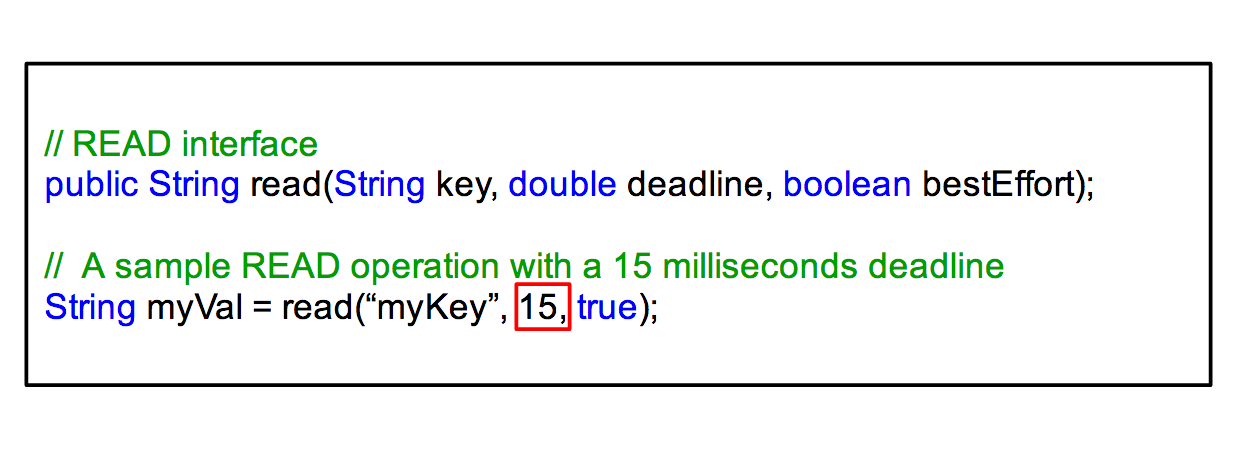
\includegraphics[scale=0.25]{img/MicroFuge_protocol.png}
  \caption{MicroFuge \textit{read} operation interface.}
    %% \end{flushleft}
  \end{figure}
\end{frame}

\begin{frame}
  \frametitle{Deadline Cache (DLC) - Components}
  \begin{figure}
    \begin{center}
      \centerline{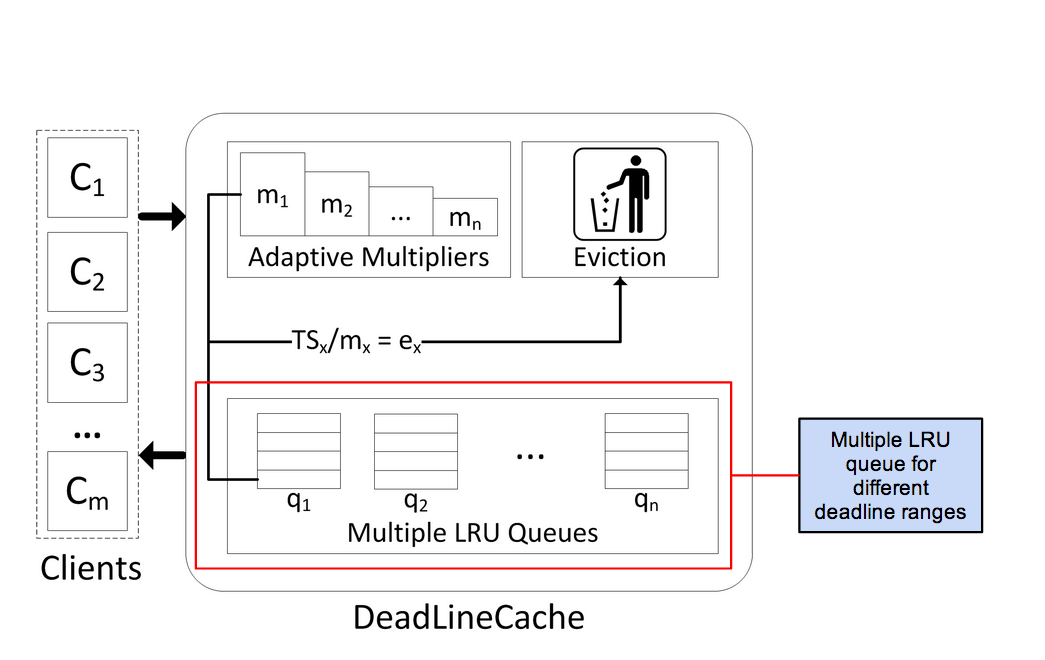
\includegraphics[scale=0.38]{img/DLC_ARC_1.png}}
    \end{center}
  \end{figure}
\end{frame}


\begin{frame}
  \frametitle{Deadline Cache (DLC) - Components}
  \begin{figure}
    \begin{center}
      \centerline{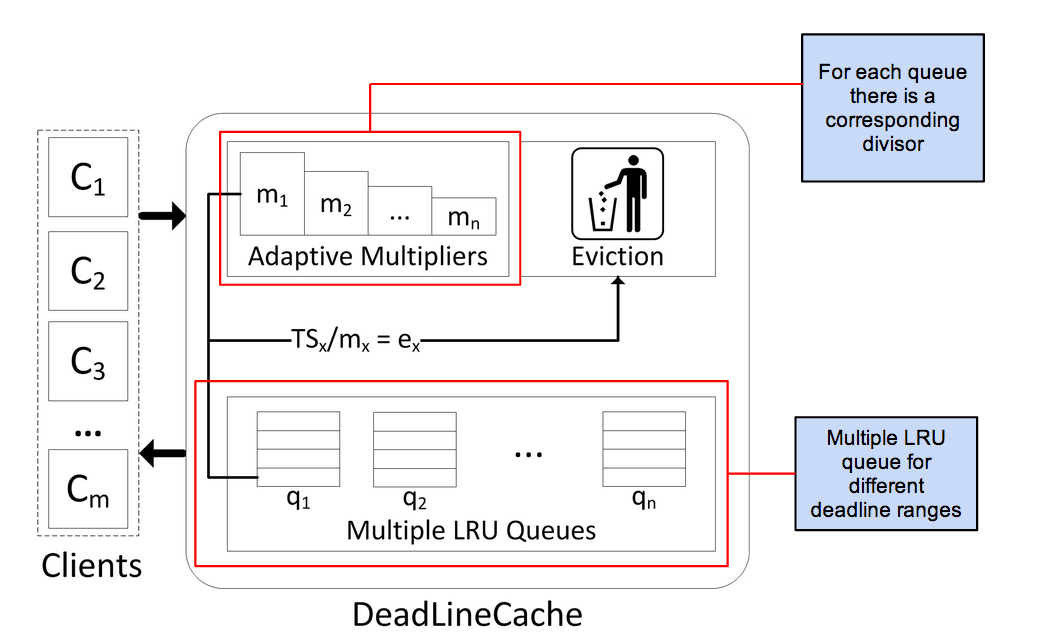
\includegraphics[scale=0.38]{img/DLC_ARC_2.png}}
    \end{center}
  \end{figure}
\end{frame}


\begin{frame}
  \frametitle{Deadline Cache (DLC) - Components}
  \begin{figure}
    \begin{center}
      \centerline{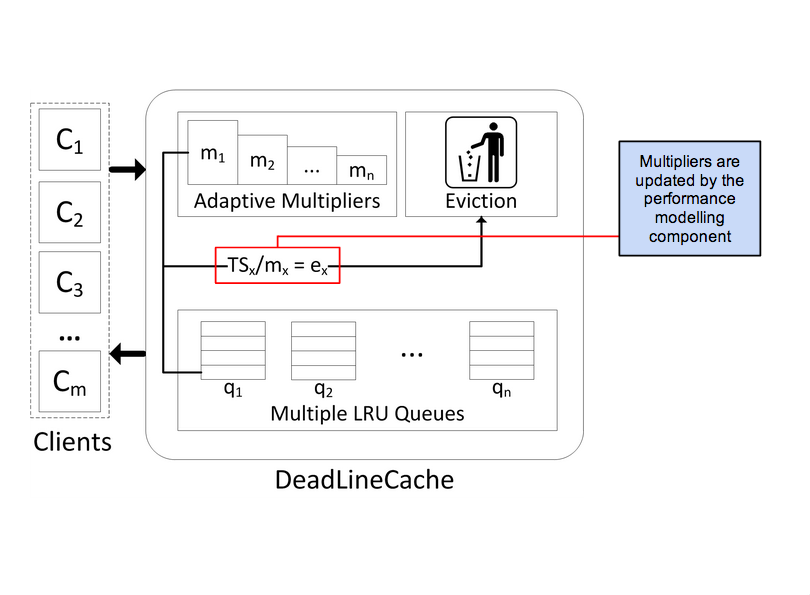
\includegraphics[scale=0.38]{img/DLC_ARC_3.png}}
    \end{center}
  \end{figure}
\end{frame}

\begin{frame}
  \frametitle{DLC - An Cache Eviction Example (0)}
  \begin{itemize}
  \item Client issues a cache lookup.
  \item Not in the cache.
  \item Client retrieves the item from the database.
  \item Client issues a cache put.
  \item If the cache is full, a cache eviction happens.
  \end{itemize}
\end{frame}

\begin{frame}
  \frametitle{DLC - An Cache Eviction Example (1)}
  \begin{figure}
    \begin{center}
      \centerline{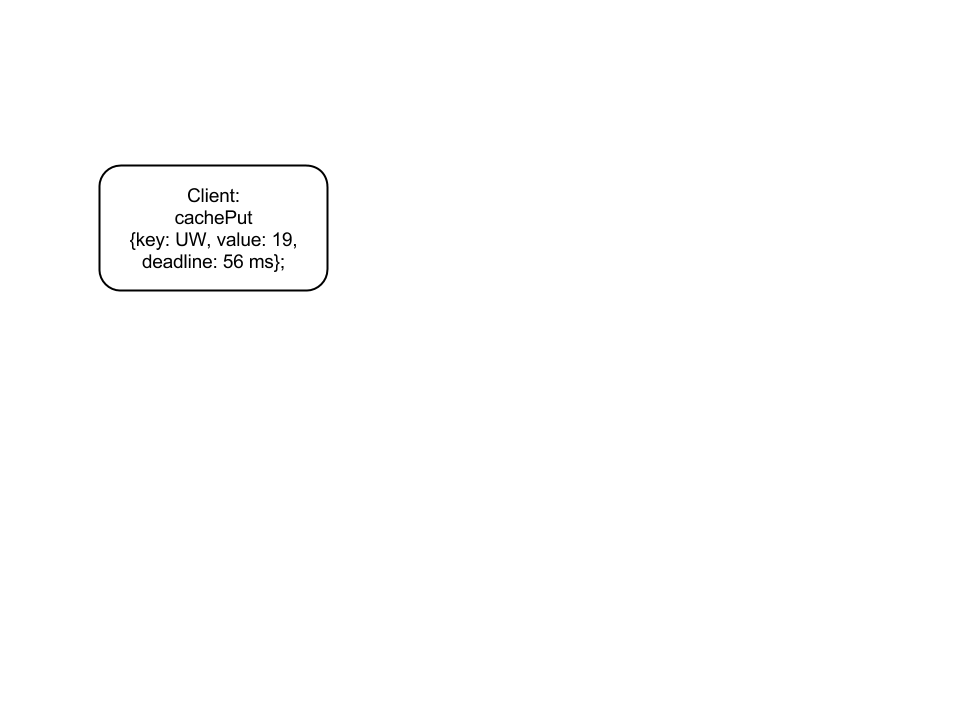
\includegraphics[scale=0.33]{img/DLC_NEW_1.png}}
    \end{center}
  \end{figure}
\end{frame}


\begin{frame}
  \frametitle{DLC - An Cache Eviction Example (2)}
  \begin{figure}
    \begin{center}
      \centerline{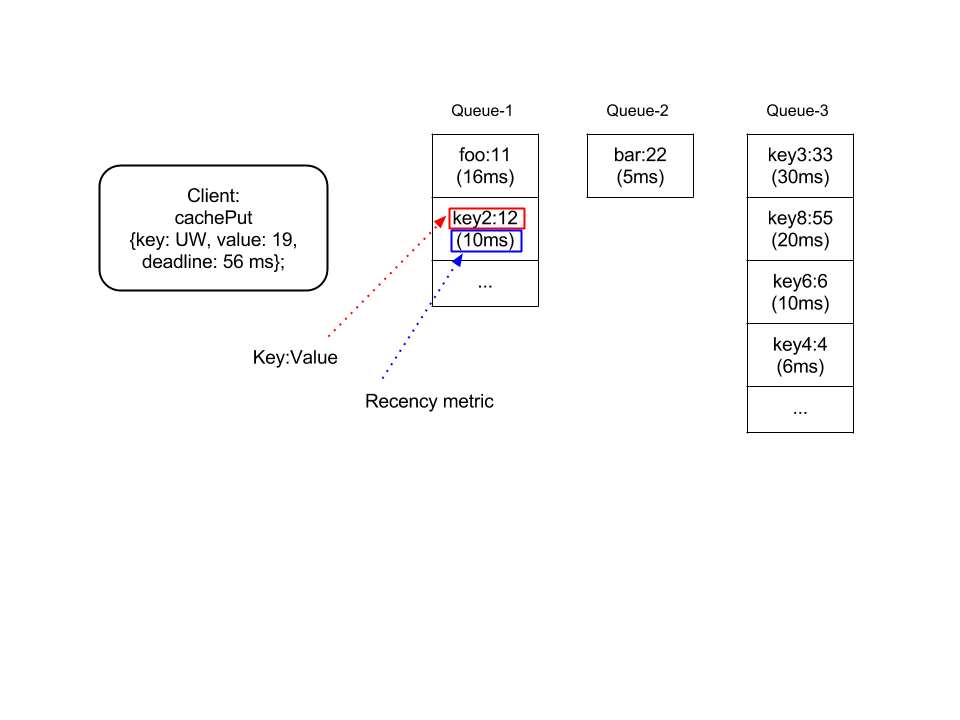
\includegraphics[scale=0.33]{img/DLC_NEW_2.png}}
    \end{center}
  \end{figure}
\end{frame}

\begin{frame}
  \frametitle{DLC - An Cache Eviction Example (3)}
  \begin{figure}
    \begin{center}
      \centerline{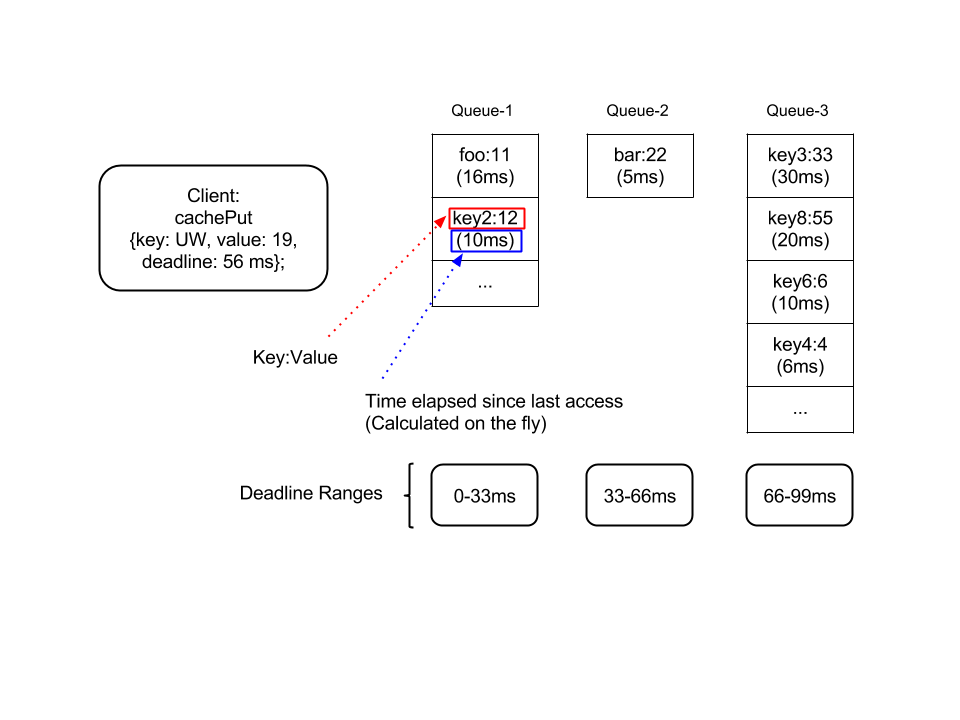
\includegraphics[scale=0.33]{img/DLC_NEW_3.png}}
    \end{center}
  \end{figure}
\end{frame}

\begin{frame}
  \frametitle{DLC - An Cache Eviction Example (4)}
  \begin{figure}
    \begin{center}
      \centerline{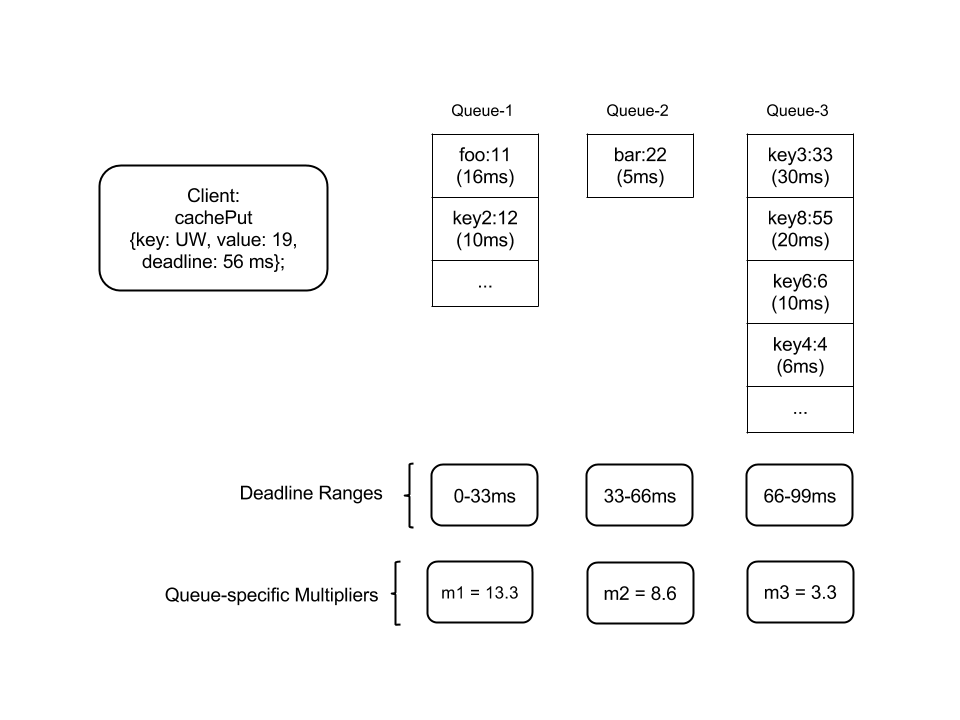
\includegraphics[scale=0.33]{img/DLC_NEW_4.png}}
    \end{center}
  \end{figure}
\end{frame}


\begin{frame}
  \frametitle{DLC - An Cache Eviction Example (5)}
  \begin{figure}
    \begin{center}
      \centerline{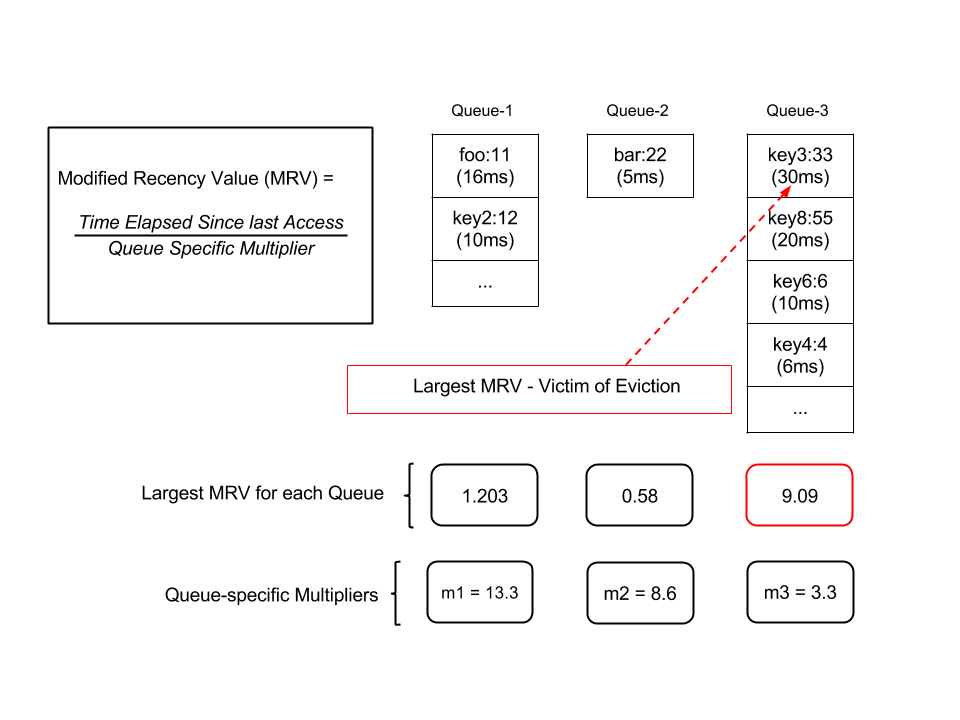
\includegraphics[scale=0.33]{img/DLC_NEW_5.png}}
    \end{center}
  \end{figure}
\end{frame}

\begin{frame}
  \frametitle{DLC - An Cache Eviction Example (6)}
  \begin{figure}
    \begin{center}
      \centerline{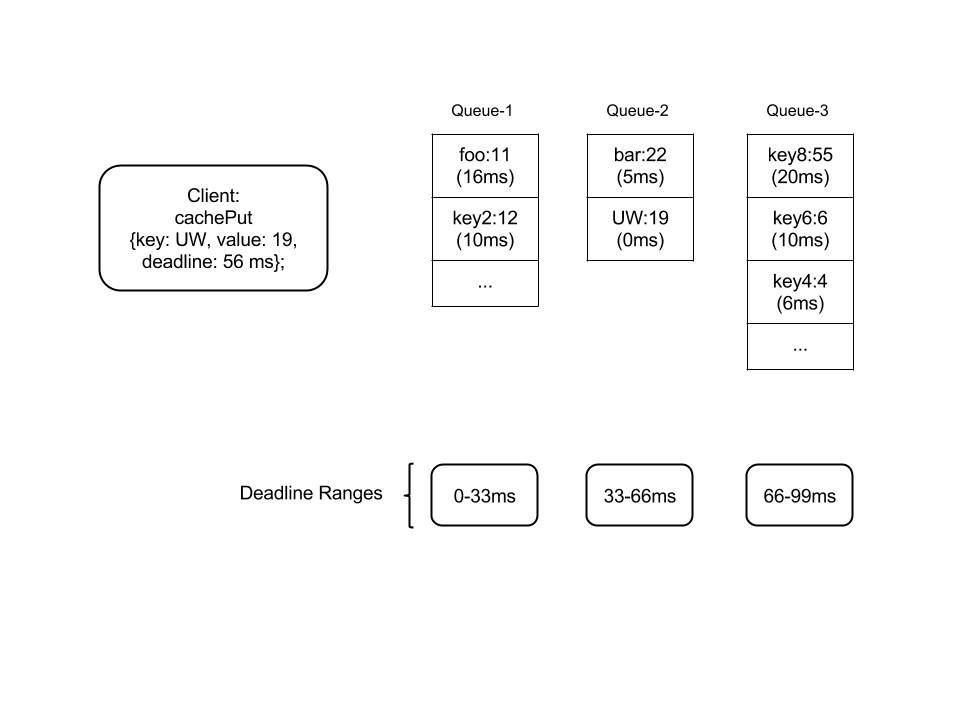
\includegraphics[scale=0.33]{img/DLC_NEW_6.png}}
    \end{center}
  \end{figure}
\end{frame}


\begin{frame}
  \frametitle{DLC - An Cache Eviction Example (7)}
  \begin{figure}
    \begin{center}
      \centerline{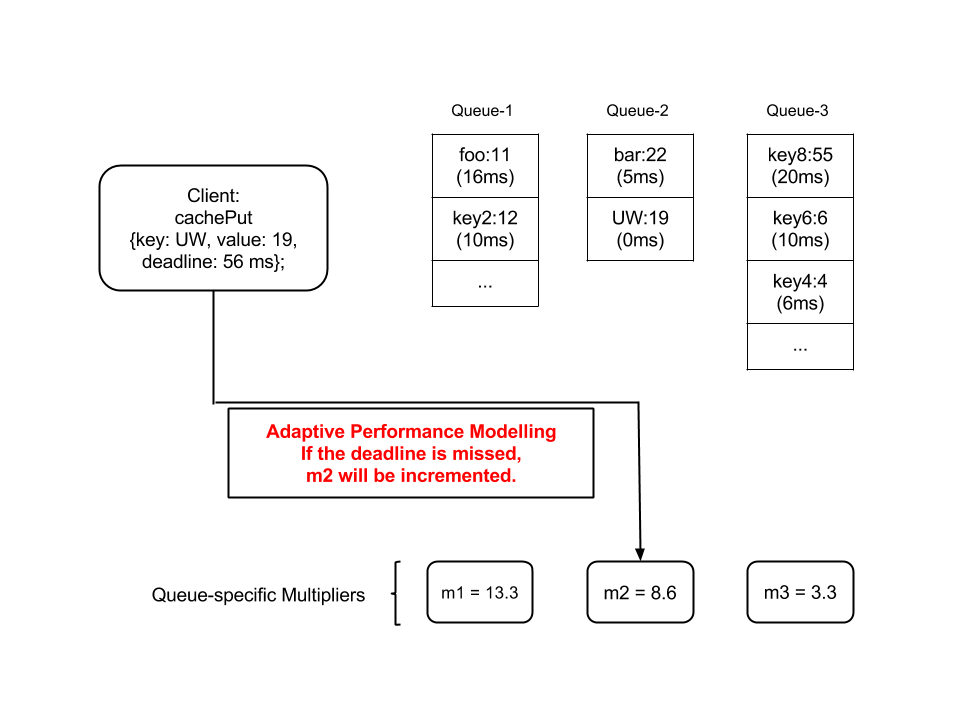
\includegraphics[scale=0.33]{img/DLC_NEW_7.png}}
    \end{center}
  \end{figure}
\end{frame}

\begin{frame}
  \frametitle{DLC - Advantages}
  \vspace{-15 mm}
  \begin{itemize}
  \item Deadline Aware.
    \myv
  \item Adaptive performance modelling.
    \begin{itemize}
      \myv
    \item Avoids overestimating or underestimating the underlying storage
      system's performance which leads to higher deadline violations.
      \myv
    \end{itemize}

  \end{itemize}
\end{frame}


\begin{frame}
  \frametitle{Deadline Scheduler (DLS) High-level Architecture}
  \begin{itemize}
  \item Each scheduler is responsible for
    controlling the access to a single data-server.
  \end{itemize}
  \begin{figure}
    \begin{center}
      \centerline{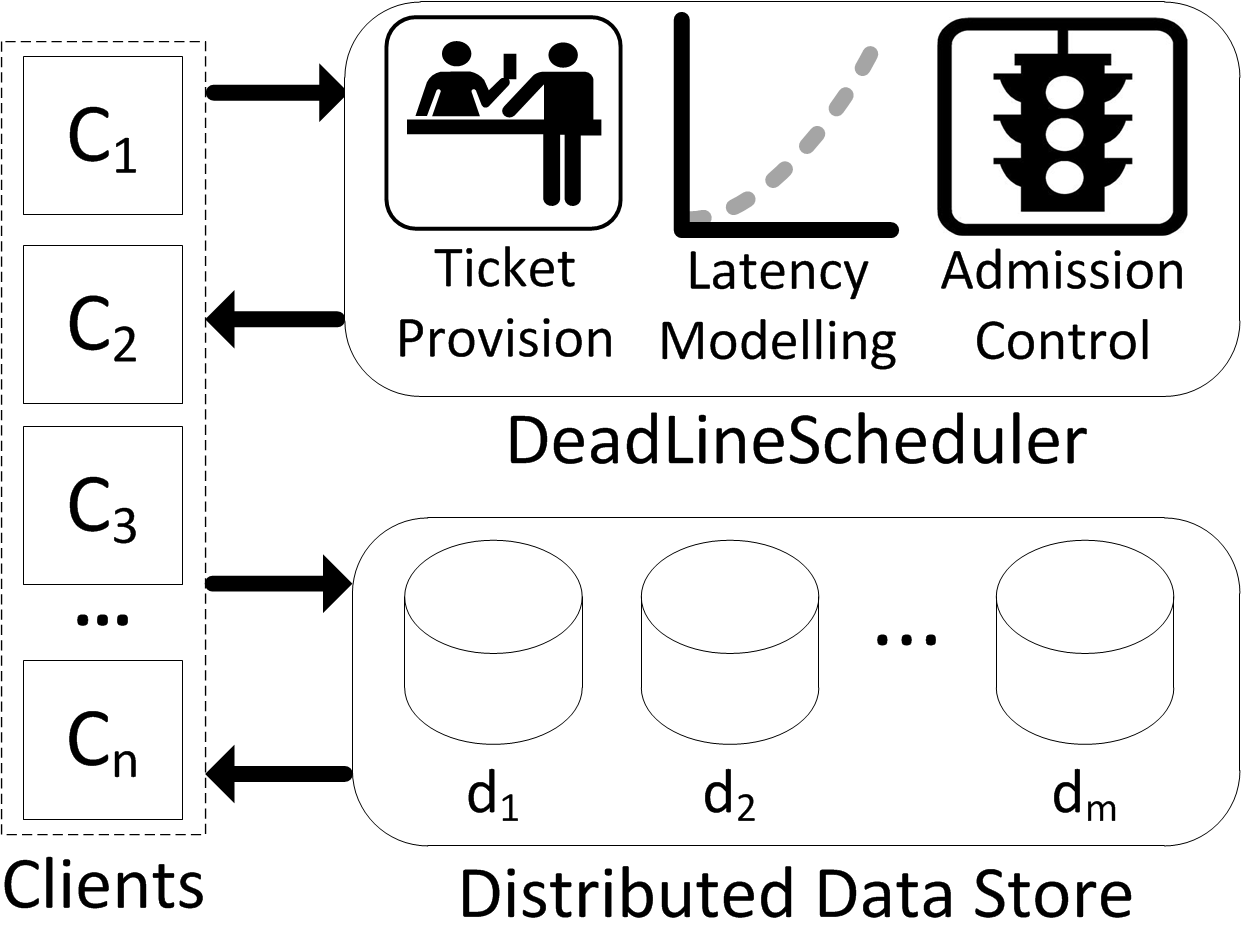
\includegraphics[scale=0.90]{img/DLS.png}}
    \end{center}
  \end{figure}
\end{frame}

\begin{frame}
  \frametitle{DLS - An Example Setup}
  \begin{itemize}
  \item Each key-value pair is replicated three times. blah blah blah
    \newline

  \end{itemize}
  \begin{figure}
    \begin{center}
      \centerline{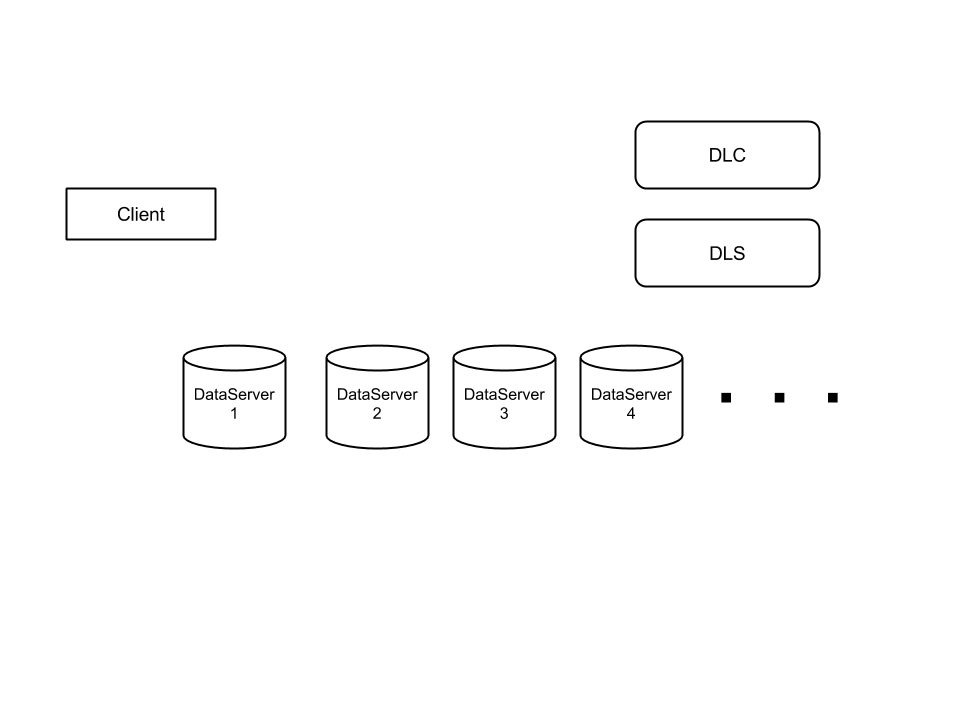
\includegraphics[scale=0.40]{img/DLS_Example1.png}}
    \end{center}
  \end{figure}

\end{frame}


\begin{frame}
  \frametitle{DLS - An Example 1}
  \begin{itemize}
  \item The client wants to perform a simple value lookup for the key UW.
  \end{itemize}
  \begin{figure}
    \begin{center}
      \centerline{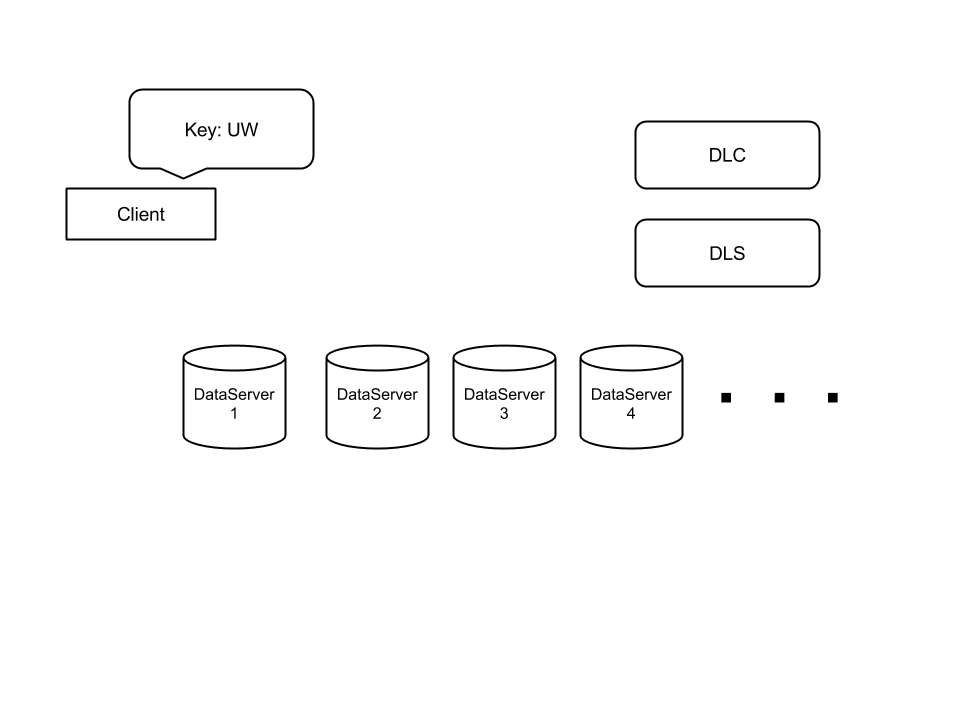
\includegraphics[scale=0.40]{img/DLS_Example2.png}}
    \end{center}
  \end{figure}
\end{frame}


\begin{frame}
  \frametitle{DLS - An Example 2}
  \begin{itemize}
  \item The client begins by issuing a cache lookup to DLC.
\newline
  \end{itemize}
  \begin{figure}
    \begin{center}
      \centerline{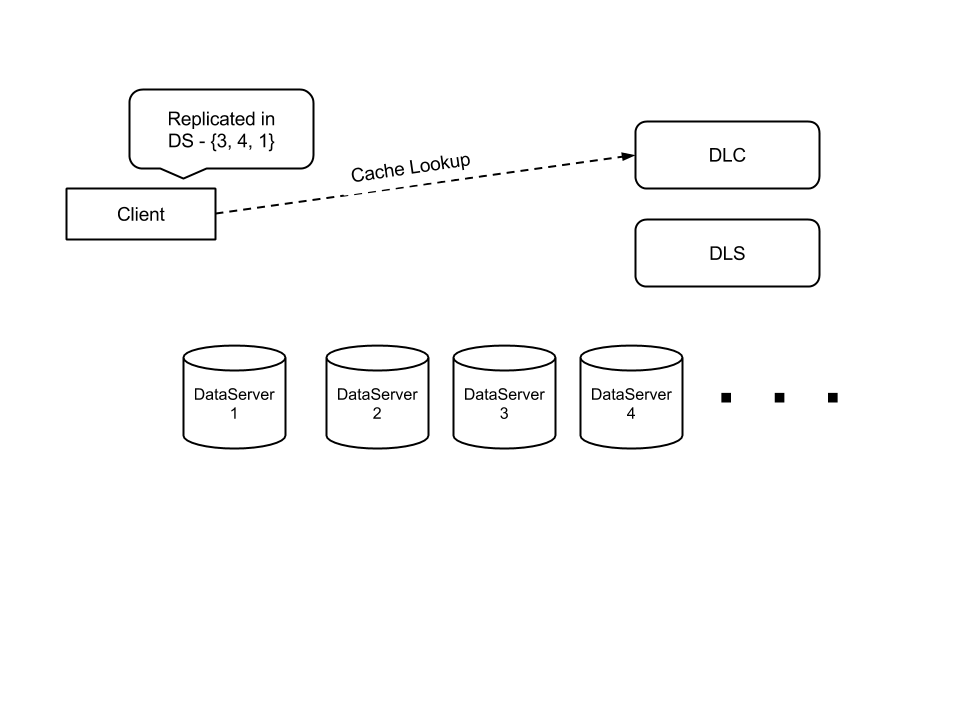
\includegraphics[scale=0.40]{img/DLS_Example3.png}}
    \end{center}
  \end{figure}


\end{frame}

\begin{frame}
  \frametitle{DLS - An Example 3}
  \begin{itemize}
  \item Issue ticket \textit{get requests} concurrently.
\newline
  \end{itemize}
  \begin{figure}
    \begin{center}
      \centerline{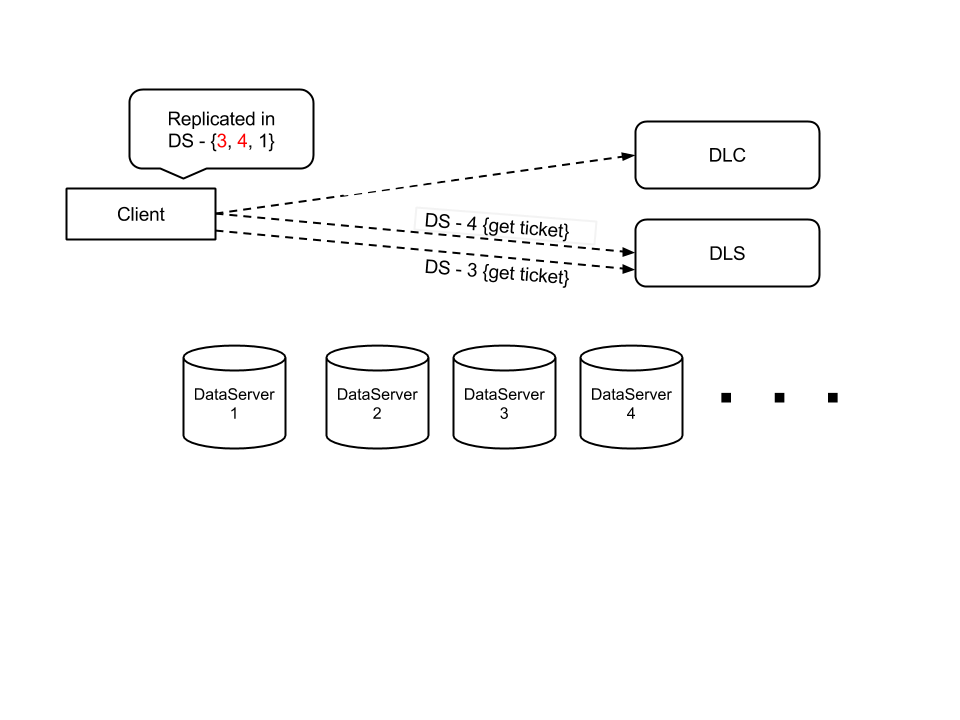
\includegraphics[scale=0.40]{img/DLS_Example4.png}}
    \end{center}
  \end{figure}

\end{frame}

\begin{frame}
  \frametitle{DLS - An Example 4}
  \begin{itemize}
  \item If the item is not in the cache, the client waits for the DLS to
    return the tickets.
  \end{itemize}
  \begin{figure}
    \begin{center}
      \centerline{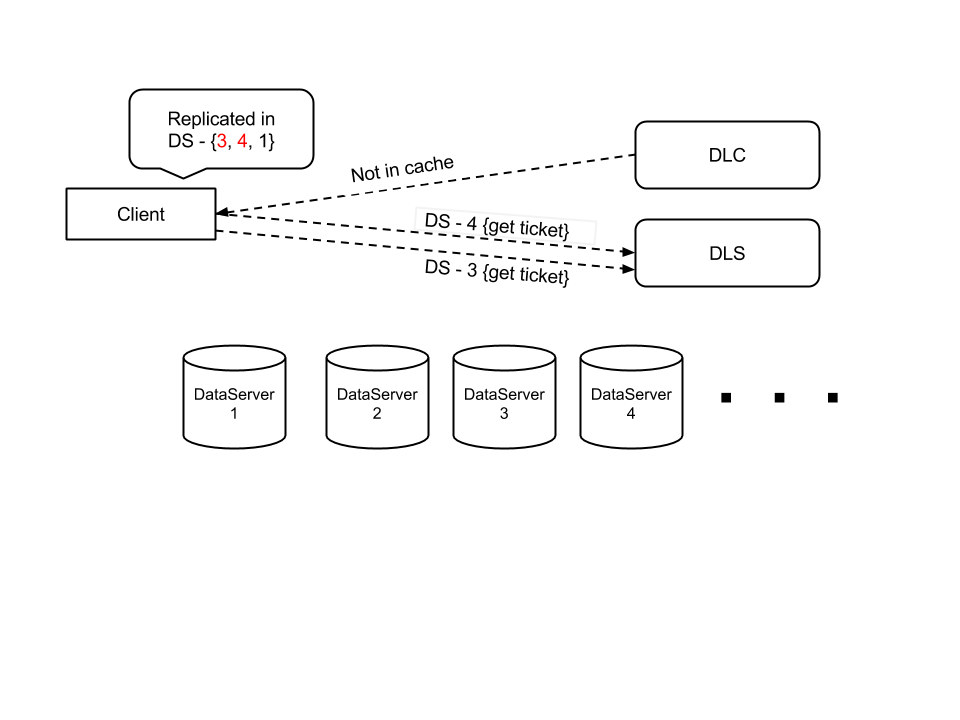
\includegraphics[scale=0.40]{img/DLS_Example5.png}}
    \end{center}
  \end{figure}

\end{frame}


\begin{frame}
  \frametitle{DLS - An Example 5}
  \begin{itemize}
  \item When the tickets are sent back to the client, the client will pick
    the DLS server which responds the first.
  \end{itemize}
  \begin{figure}
    \begin{center}
      \centerline{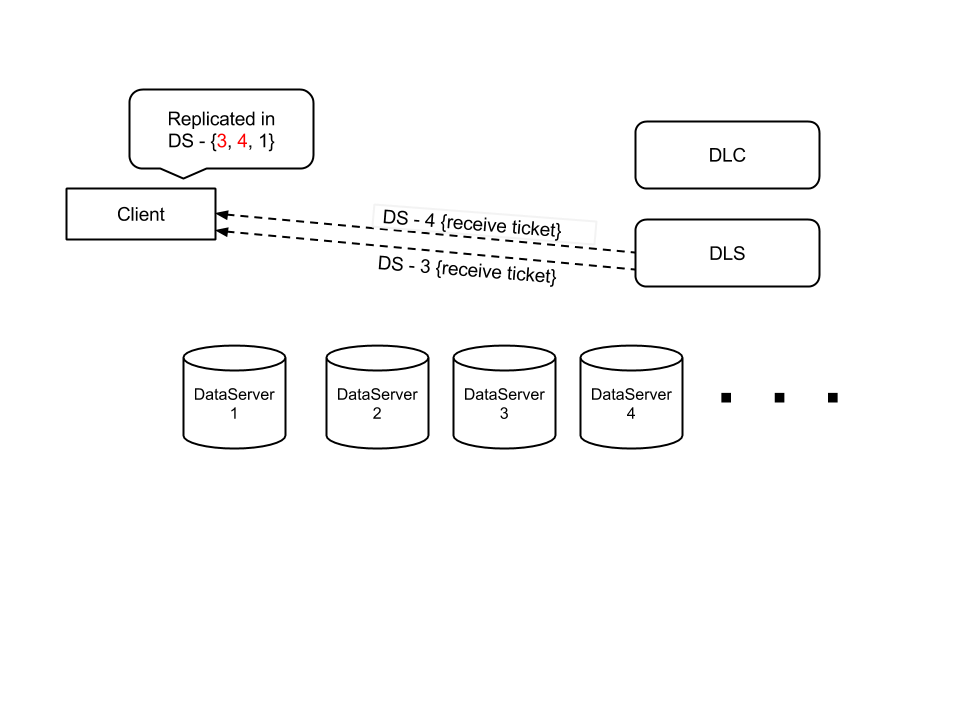
\includegraphics[scale=0.40]{img/DLS_Example6.png}}
    \end{center}
  \end{figure}

\end{frame}

\begin{frame}
  \frametitle{DLS - An Example 6}
  \begin{itemize}
  \item The client makes a blocking call to the selected DLS and waits for
    its turn to access the data server.
  \end{itemize}
  \begin{figure}
    \begin{center}
      \centerline{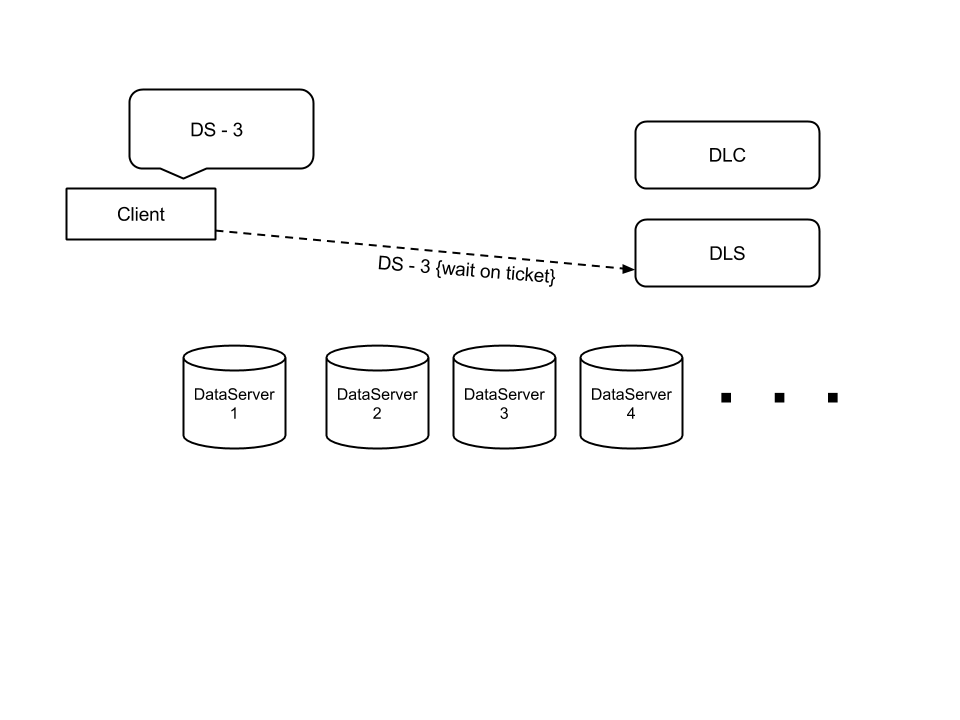
\includegraphics[scale=0.40]{img/DLS_Example7.png}}
    \end{center}
  \end{figure}

\end{frame}

\begin{frame}
  \frametitle{DLS - An Example 7}
  \begin{itemize}
  \item The client's request is inserted into DLS's pending queue.
\newline
  \end{itemize}
  \begin{figure}
    \begin{center}
      \centerline{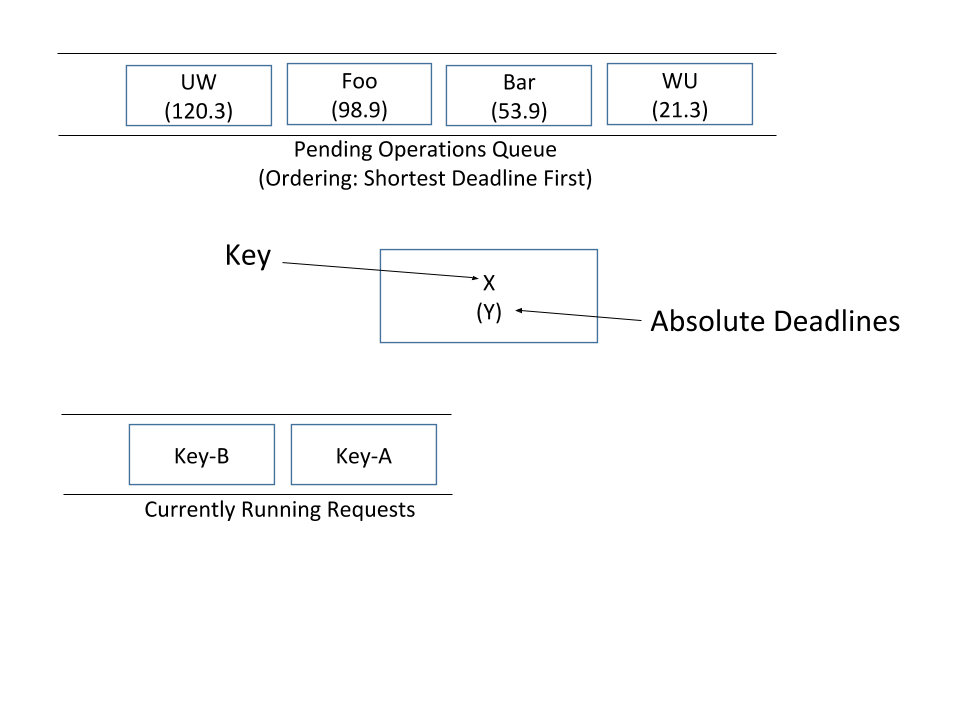
\includegraphics[scale=0.38]{img/DLS_Example8.png}}
    \end{center}
  \end{figure}

\end{frame}

\begin{frame}
  \frametitle{DLS - An Example 8}
  \begin{itemize}
  \item When a request leaves the pending queue, the DLS may increase the
    request's deadline and insert the request back into the queue if the
    deadline can not be met.
  \end{itemize}
  \begin{figure}
    \begin{center}
      \centerline{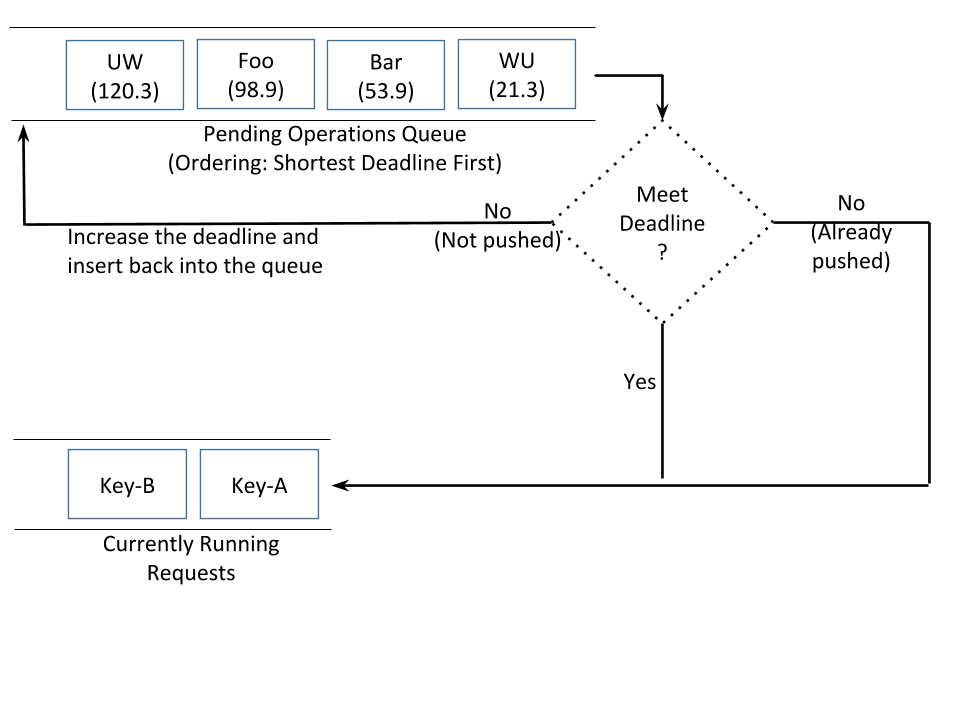
\includegraphics[scale=0.33]{img/DLS_Example9.png}}
    \end{center}
  \end{figure}


\end{frame}

\begin{frame}
  \frametitle{DLS - An Example 9}
  \begin{itemize}
  \item The DLS informs the client that the wait is over.
\newline
  \end{itemize}
  \begin{figure}
    \begin{center}
      \centerline{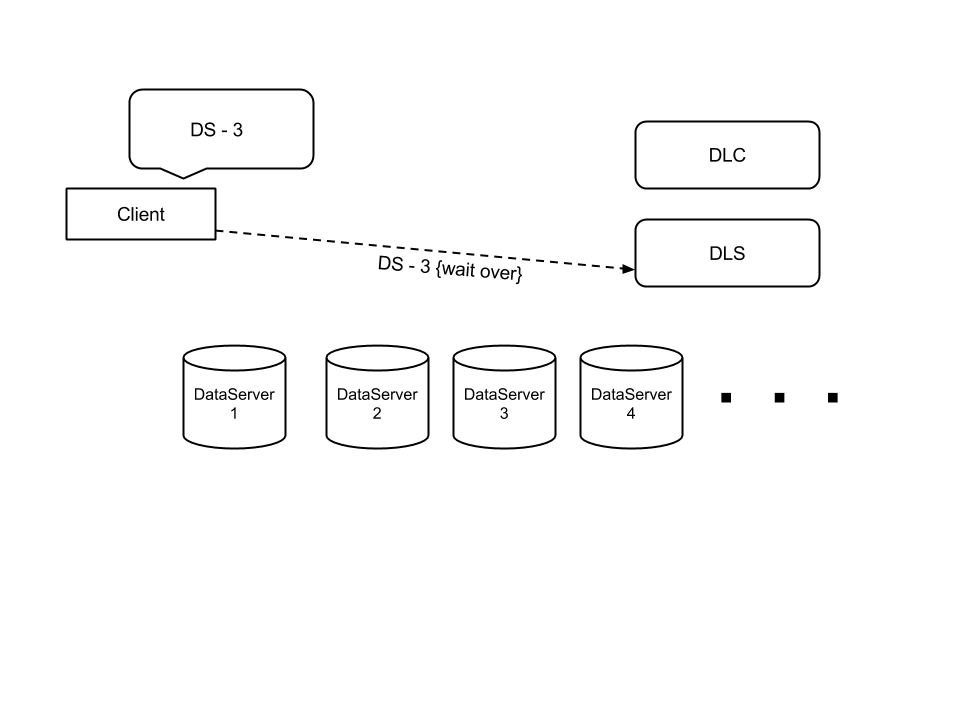
\includegraphics[scale=0.35]{img/DLS_Example10.png}}
    \end{center}
  \end{figure}
\end{frame}


\begin{frame}
  \frametitle{DLS - An Example 10}
  \begin{itemize}
  \item The clients issues the read request to the data server.
\newline
  \end{itemize}
  \begin{figure}
    \begin{center}
      \centerline{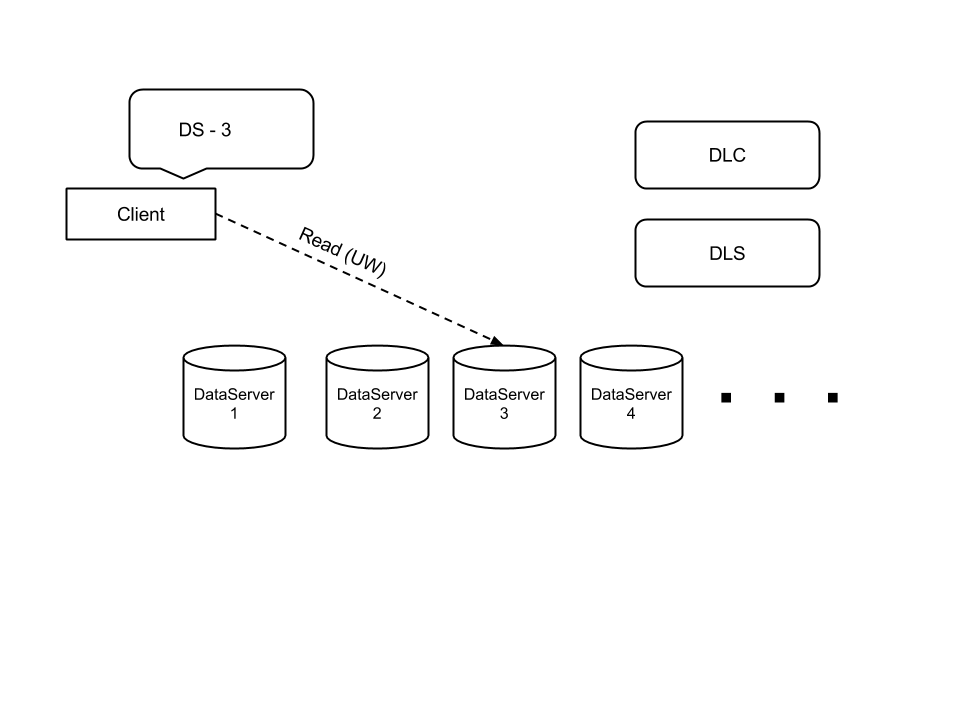
\includegraphics[scale=0.35]{img/DLS_Example11.png}}
    \end{center}
  \end{figure}

\end{frame}

\begin{frame}
  \frametitle{DLS - An Example 11}
  \begin{itemize}
  \item After receiving the response, the client releases
    the ticket and concurrently inserts the data into the cache.
  \end{itemize}
  \begin{figure}
    \begin{center}
      \centerline{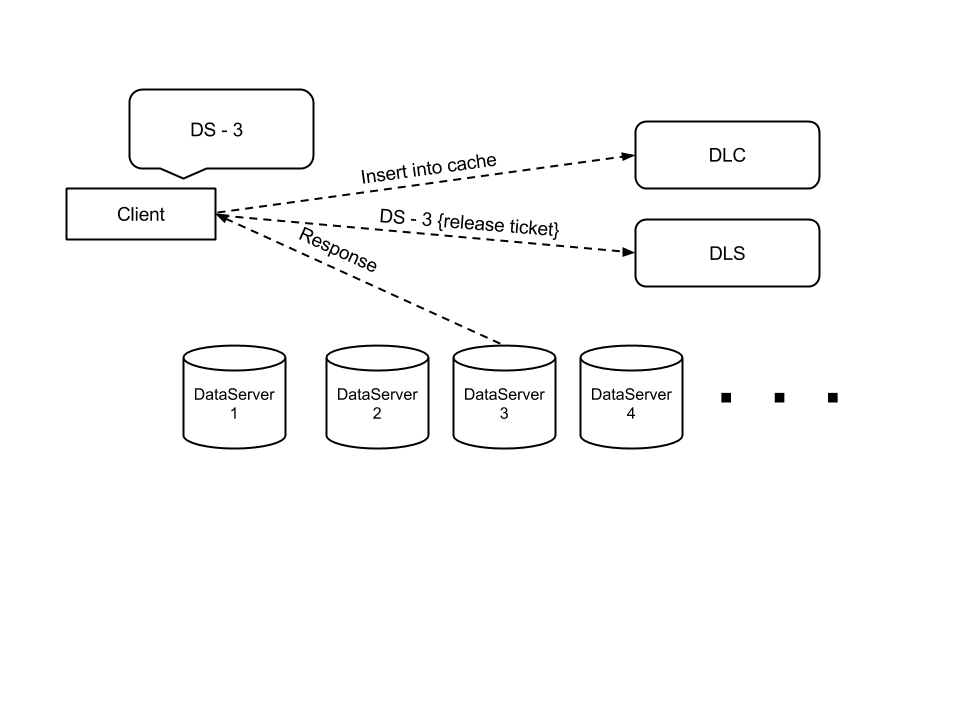
\includegraphics[scale=0.35]{img/DLS_Example12.png}}
    \end{center}
  \end{figure}

\end{frame}


\begin{frame}
  \frametitle{DLS - Admission Control}
  \begin{itemize}
  \item Bound the fraction of requests that miss their deadlines.
  \item Requests are rejected in two situations.
    \begin{itemize}
    \item The request will be miss its own deadline.
    \item The new request will cause already accepted requests to miss their deadlines.
    \end{itemize}
  \item Provides a system parameter $\beta$ as a knob to control the percentage
    of deadline misses.
  \end{itemize}
\end{frame}

\begin{frame}
  \frametitle{Full MicroFuge}
  \begin{itemize}
  \item
    MicroFuge combines both the DLC and DLS layers to achieve its best
    performance.
  \end{itemize}

  \begin{figure}
    \begin{center}
      \centerline{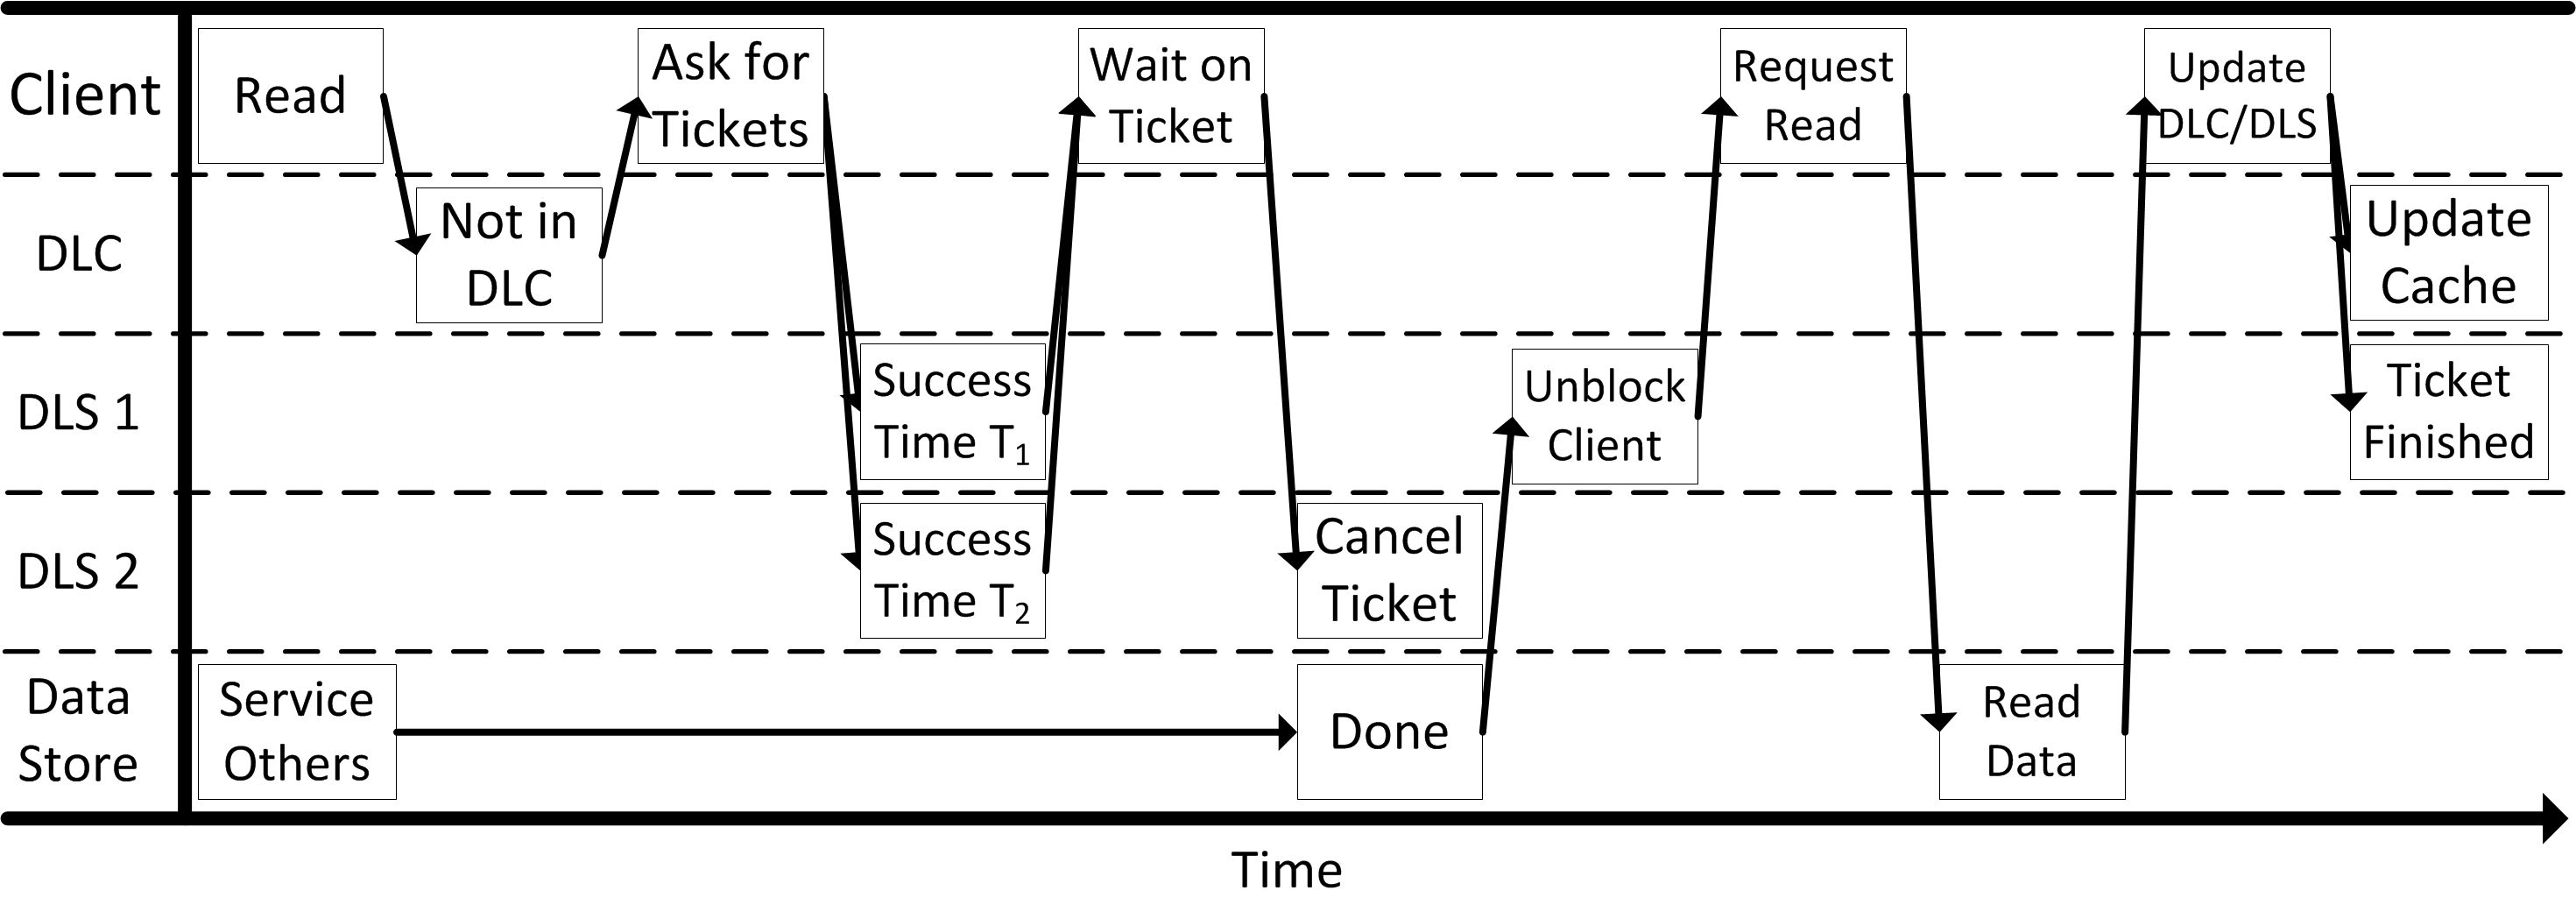
\includegraphics[scale=0.60]{img/RequestTimelineHorizontal.png}}
    \end{center}
  \end{figure}
\end {frame}



\begin{frame}
  \frametitle{Goals of the Evaluation}
  \begin{itemize}
  \item Comparison of the two caching systems.
    \begin{itemize}
    \item Deadline Cache
    \item Memcached
    \end{itemize}
  \item Effectiveness of MicroFuge.
    \begin{itemize}
    \item Caching Layer
    \item Scheduling layer
    \item Admission control
    \end{itemize}
  \end{itemize}
\end{frame}


\begin{frame}
  \frametitle{Experimental Setup - The Cluster}
  \begin{itemize}
  \item Twenty-node test cluster on AWS. Each cluster node is an m1.medium
    EC2 instance.
  \end{itemize}
  \begin{figure}
    \begin{center}
      \centerline{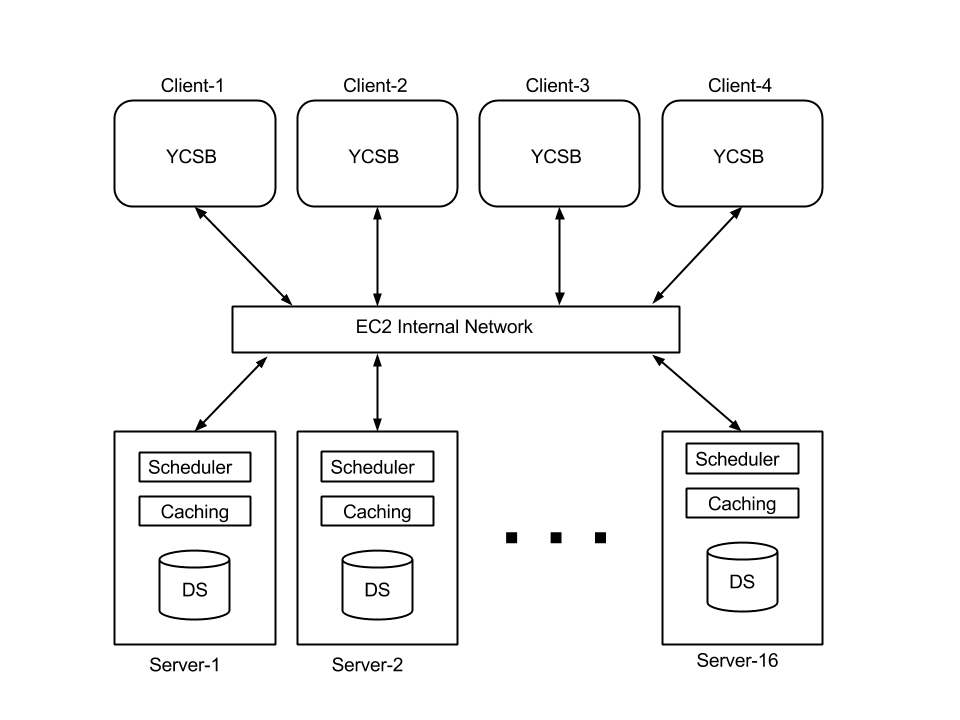
\includegraphics[scale=0.25]{img/Experimental_Setup.png}}
    \end{center}
  \end{figure}
\end{frame}

\begin{frame}
  \frametitle{Experimental Setup - Details}
  \begin{itemize}
  \item DataServer - Simple key-value store that uses leveldb with a
    replication factor 3.
  \item Benchmarking System - Modified version of Yahoo! Cloud Serving
    Benchmark (YCSB).
    \begin{itemize}
    \item Assign deadlines to each key.\\
      %% \begin{center}
      \begin{tabular}{| l | c |}
        \hline
        Range & Percentage \\ \hline
        10-30ms & 20\% \\ \hline
        30-100ms & 30\% \\ \hline
        100-1000ms & 50\% \\ \hline
      \end{tabular}
      %% \end{center}
    \end{itemize}
  \item Data Set - Key-value store with 80 million records, 86.4 GB in size.
  \item Cache - Total capacity of 19.2GB.
  \end{itemize}
\end{frame}


\begin{frame}
  \frametitle{Experimental Results - Deadline-Aware Caching 1}
  \begin{figure}[t]
    \begin{center}
      \centerline{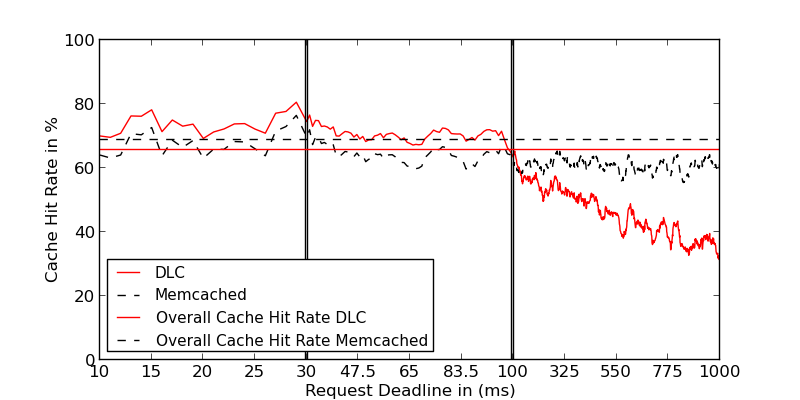
\includegraphics[scale=0.5]{img/EC2/EC2_CS_MM/cache_48.png}}
      \caption{Cache hit rate for 192 concurrent clients with DLC and Memcached.}
      \label{fig:cache_192_cs_mm}
    \end{center}
  \end{figure}
\end{frame}

\begin{frame}
  \frametitle{Experimental Results - Deadline-Aware Caching 2}
  \begin{figure}[t]
    \begin{center}
      \centerline{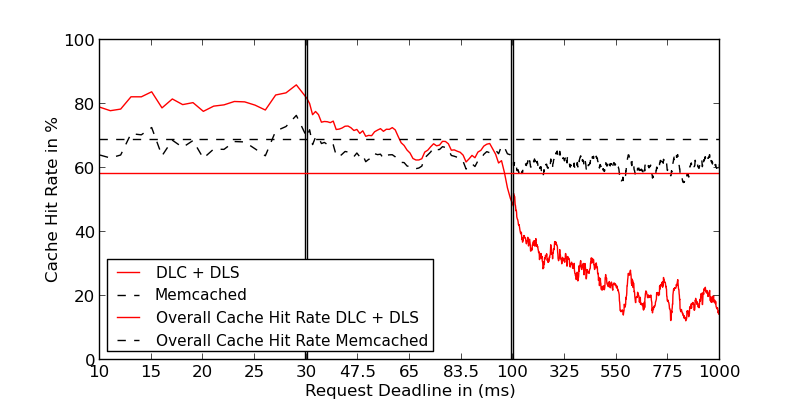
\includegraphics[scale=0.5]{img/EC2/EC2_SH_MM/cache_48.png}}
      \caption{Cache hit rate for 192 concurrent clients with DLC + DLS and Memcached.}
      \label{fig:cache_192_sh_mm}
    \end{center}
  \end{figure}
\end{frame}




\begin{frame}
  \frametitle{Experimental Results - Deadline Miss 1}
  \begin{figure}[t]
    \begin{center}
      \centerline{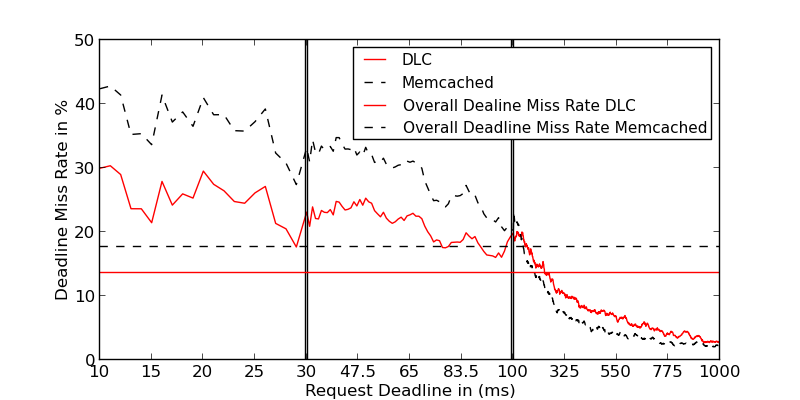
\includegraphics[scale=0.5]{img/EC2/EC2_CS_MM/miss_48.png}}
      \caption{Deadline miss rate for 192 concurrent clients with DLC and Memcached.}
      \label{fig:miss_192_cs_mm}
    \end{center}
  \end{figure}
\end{frame}


\begin{frame}
  \frametitle{Experimental Results - Deadline Miss 2}
  \begin{figure}[t]
    \begin{center}
      \centerline{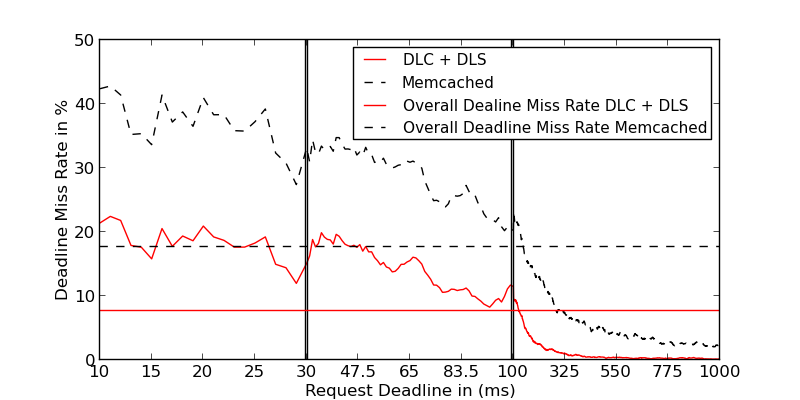
\includegraphics[scale=0.5]{img/EC2/EC2_SH_MM/miss_48.png}}
      \caption{Deadline miss rate for 192 concurrent clients with DLC + DLS and Memcached.}
      \label{fig:miss_192_sh_mm}
    \end{center}
  \end{figure}
\end{frame}

\begin{frame}
  \frametitle{Experimental Results - Deadline Miss 3}
  \begin{figure}[t]
    \begin{center}
      \centerline{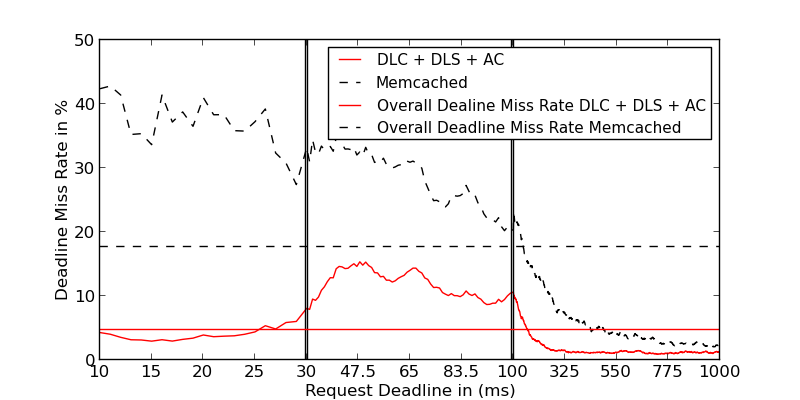
\includegraphics[scale=0.5]{img/EC2/EC2_AC_MM/miss_48.png}}
      \caption{Deadline miss rate for 192 concurrent clients with DLC + DLS + AC and Memcached.}
      \label{fig:miss_192_ac_mm}
    \end{center}
  \end{figure}
\end{frame}

\begin{frame}
  \frametitle{Experimental Results - Tunable Admission Control}
  \begin{figure}[t]
    \begin{center}
      \centerline{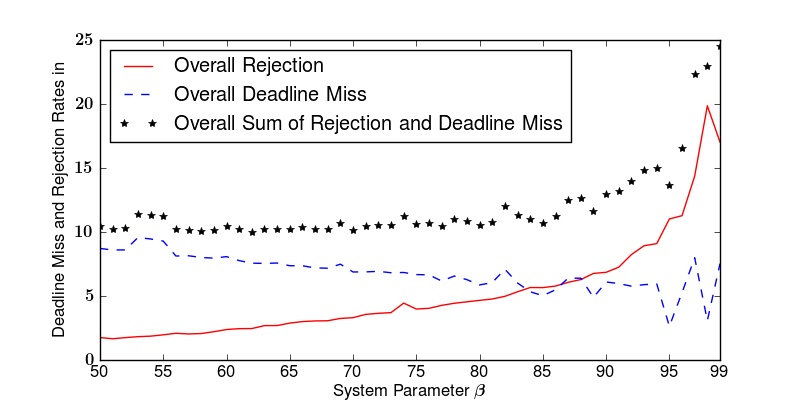
\includegraphics[scale=0.5]{img/EC2/Varying_ac/varying_acPerc_192.png}}
      \caption{Deadline miss vs. rejection rates with respect to various values of
        system parameter $\beta$ for 192 clients.}
      \label{fig:varying_ac}
    \end{center}
  \end{figure}
\end{frame}


\begin{frame}
  \frametitle{Experimental Results - Overall Miss Rates}
  \begin{figure}[t]
    \begin{center}
      \centerline{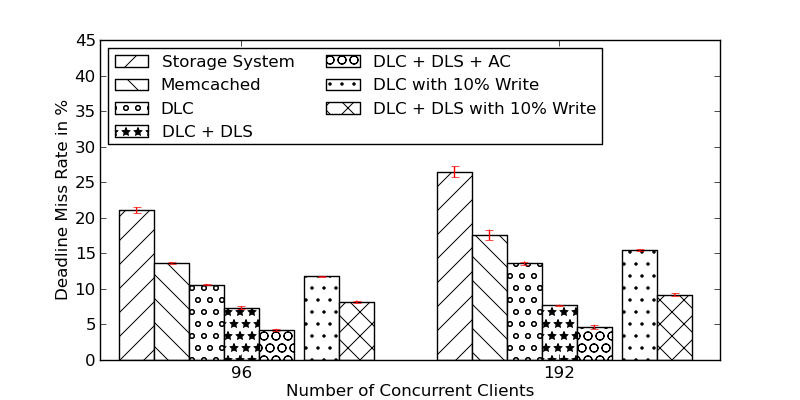
\includegraphics[scale=0.5]{img/EC2/EC2_BAR/miss_bar.png}}
      \caption{Overall deadline miss rate with various system setups for
        96 and 192 concurrent clients.}
      \label{fig:bar_miss}
    \end{center}
  \end{figure}
\end{frame}

\begin{frame}
  \frametitle{Conclusion}
  \begin{itemize}
  \item Predictable performance is necessary in multi-tenant environments.
  \item MicroFuge - A middleware approach to performance isolation in cloud
    storage systems.
  \item Deadline awareness - Reduces deadline miss rate from over 20\% to
    less than 5\%.
  \end{itemize}
\end{frame}

\end{document}
